% Preamble
\documentclass{article}

% Packages
\usepackage[T1]{fontenc} % Fontes T1
\usepackage[utf8]{inputenc} % Input UTF8
\usepackage[backend=biber, style=ieee]{biblatex} % para usar bibliografia
\usepackage{csquotes}
\usepackage[portuguese]{babel} %Usar língua portuguesa
\usepackage{blindtext}
\usepackage{graphicx} % Gerar texto automaticamente
\usepackage{geometry}
\usepackage{float}
\usepackage{hyperref}
\usepackage{indentfirst}
\usepackage[printonlyused]{acronym}
\usepackage{ragged2e}
\usepackage{textcomp}
\usepackage{multicol}

% Document
\begin{document}
    % Define keybinds
    \def\title{\textbf{MÁQUINA DE FAZER PÃO(versão 1)}}
    \def\authorjp{João Bastos (113470)}
    \def\authorrg{Rúben Gomes (113435)}
    \def\authors{João Bastos (113470), Rúben Gomes(113435)}
    \def\contacts{(113470) joaop.bastos@ua.pt, (113435) rlcg@ua.pt}
    \def\department{Departamento de Eletrónica, Telecomunicações e Informática}
    \def\university{Universidade de Aveiro}


    % Header
    \fancyhead{
        \begin{center}
            
\includegraphics{ua}\\
            \textbf{{\LARGE \title}}\\
            \vspace{2mm}
            \large Trabalho realizado por: \authors.\\
        \end{center}
    }

    % Introduction
    \section{Introdução}\label{sec:introducao}
        \par Este projeto visa implementar uma máquina de fazer pão, que permita ao utilizador escolher o tipo de pão que pretende fazer. \ Para tal, é necessário que o programa tenha uma máquina de estados finitos que permita ao utilizador escolher o tipo de pão a ser fabricado facilmente, bem como adicionar tempo extra de cozedura e/ou tempo prévio de espera para iniciar a máquina.\\

        Para tornar este projeto possível, pretendemos implementar uma máquina de estados, e os seus componentes necessários em linguagem de \textit{hardware} \acs{vhdl} e desenvolvido no software Quartus\textregistered Prime, de forma a aplicar a matéria lecionada na cadeira de \acs{lsd}.

    % Architecture
    \section{Arquitetura}\label{sec:arquitetura}
        \par A arquitetura deste projeto é divisível em várias partes distintas, que, logicamente, são complementares para o resultado do projeto. \ Estas serão descritas abaixo da Figura~\ref{fig:bread-machine}. \\

        \begin{figure}[H]
            \label{fig:bread-machine}
            \centering
            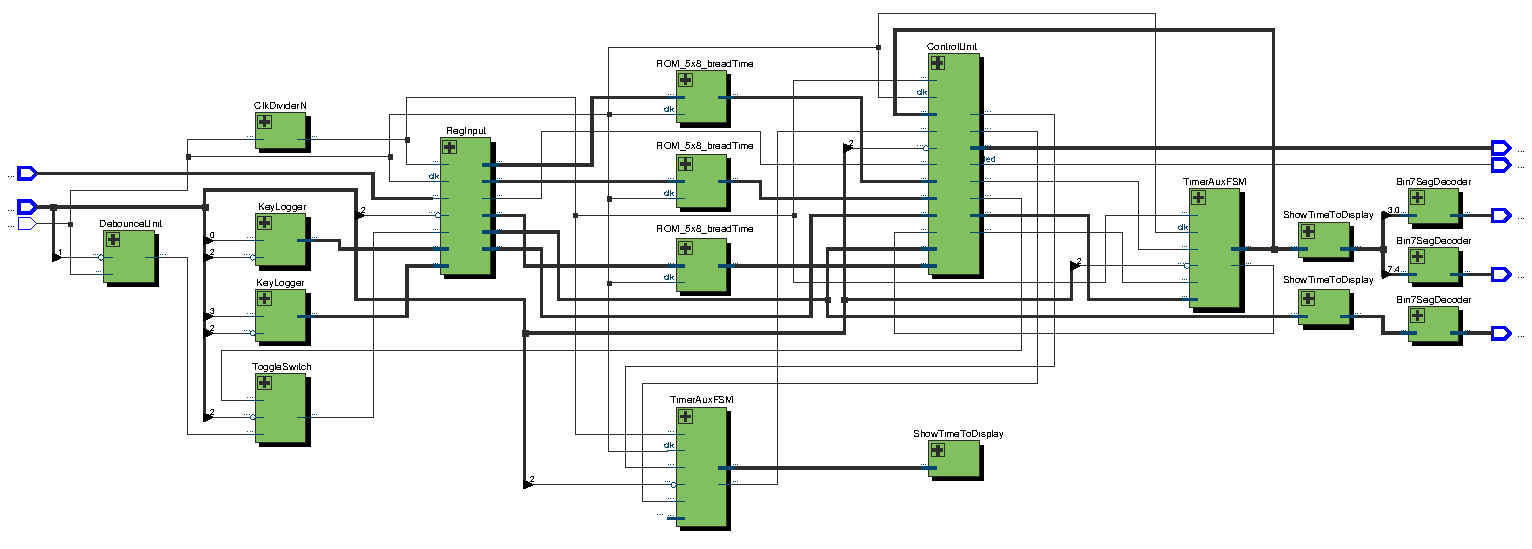
\includegraphics[scale=0.6]{BreadMachine3}
            \caption{Figura representativa do \textit{top-level} do projeto}
        \end{figure}

        \begin{itemize}
            \item[\textbf{\textrightarrow}] \textbf{KeyLogger} - Este bloco é responsável por um simples registo de cliques em um dado botão, ou seja, ao clicar uma vez, é registado esse clique como uma unidade de tempo de espera ou extra.
            \item[\textbf{\textrightarrow}] \textbf{ToggleSwitch} - O componente ToggleSwitch é usado para começar/parar a máquina de pão a qualquer momento, simulando um \textit{switch}.
            \item[\textbf{\textrightarrow}] \textbf{ClkDividerN} - Este componente é responsável por dividir o sinal de \textit{clock} por um determinado valor, de forma a que seja enviado um puslo  de um certo valor de Hertz. \ Por motivos de estar em causa um temporizador, este tem de ser dividido de forma a gerar um pulso de 1 Hz.
            \item[\textbf{\textrightarrow}] \textbf{DebounceUnit} - O seguinte componente é usado para controlar o uso de um botão. \ Um botão em uma FPGA manda centenas de sinais ao ser clicada. \ Ao usar este componente, é possível controlar o número de sinais enviados, de forma a que o botão seja ativado apenas uma vez, sem repetições.
            \item[\textbf{\textrightarrow}] \textbf{ROM\_5x8\_breadTime} - É uma memória que armazena 5 palavras de 8 bits, sendo cada palavra o tempo de um programa (como tempo de cozedura de pão rústico, por exemplo), que serão enviados para a State Machine(mais sobre a mesma na Figura~\ref{finite-states})
            \item[\textbf{\textrightarrow}] \textbf{ShowTimeToDisplay} - O seguinte bloco tem como proveito receber uma palavra de 8 bits, neste caso de um temporizador, e convertê-la em dois vetores \textit{standard logic} de 4 bits, sendo um vetor o valor das dezenas, e outro o valor das unidades, e enviá-lo para um descodificador de um \textit{display} de 7 segmentos.
            \item[\textbf{\textrightarrow}] \textbf{Bin7SegDecoder} - Este bloco descodifica uma palavra de 4 bits para um \textit{display} de 7 segmentos, de forma a que seja possível mostrar o valor decimal.
        \end{itemize}

    % Implementation
    \newpage
    \section{Implementação}\label{sec:implementacao}
        Como referido anteriormente, este projeto é maioritariamente focado em uma máquina de estados finitos, mais especificamente uma máquina de Mealy, pois depende do estado atual, como das entradas. \ Na Figura~\ref{fig:fsm}, está representado o diagrama de estados da respetiva máquina, e na lista abaixo estão descritos os seus estados.

    \begin{figure}[H]
        \centering
        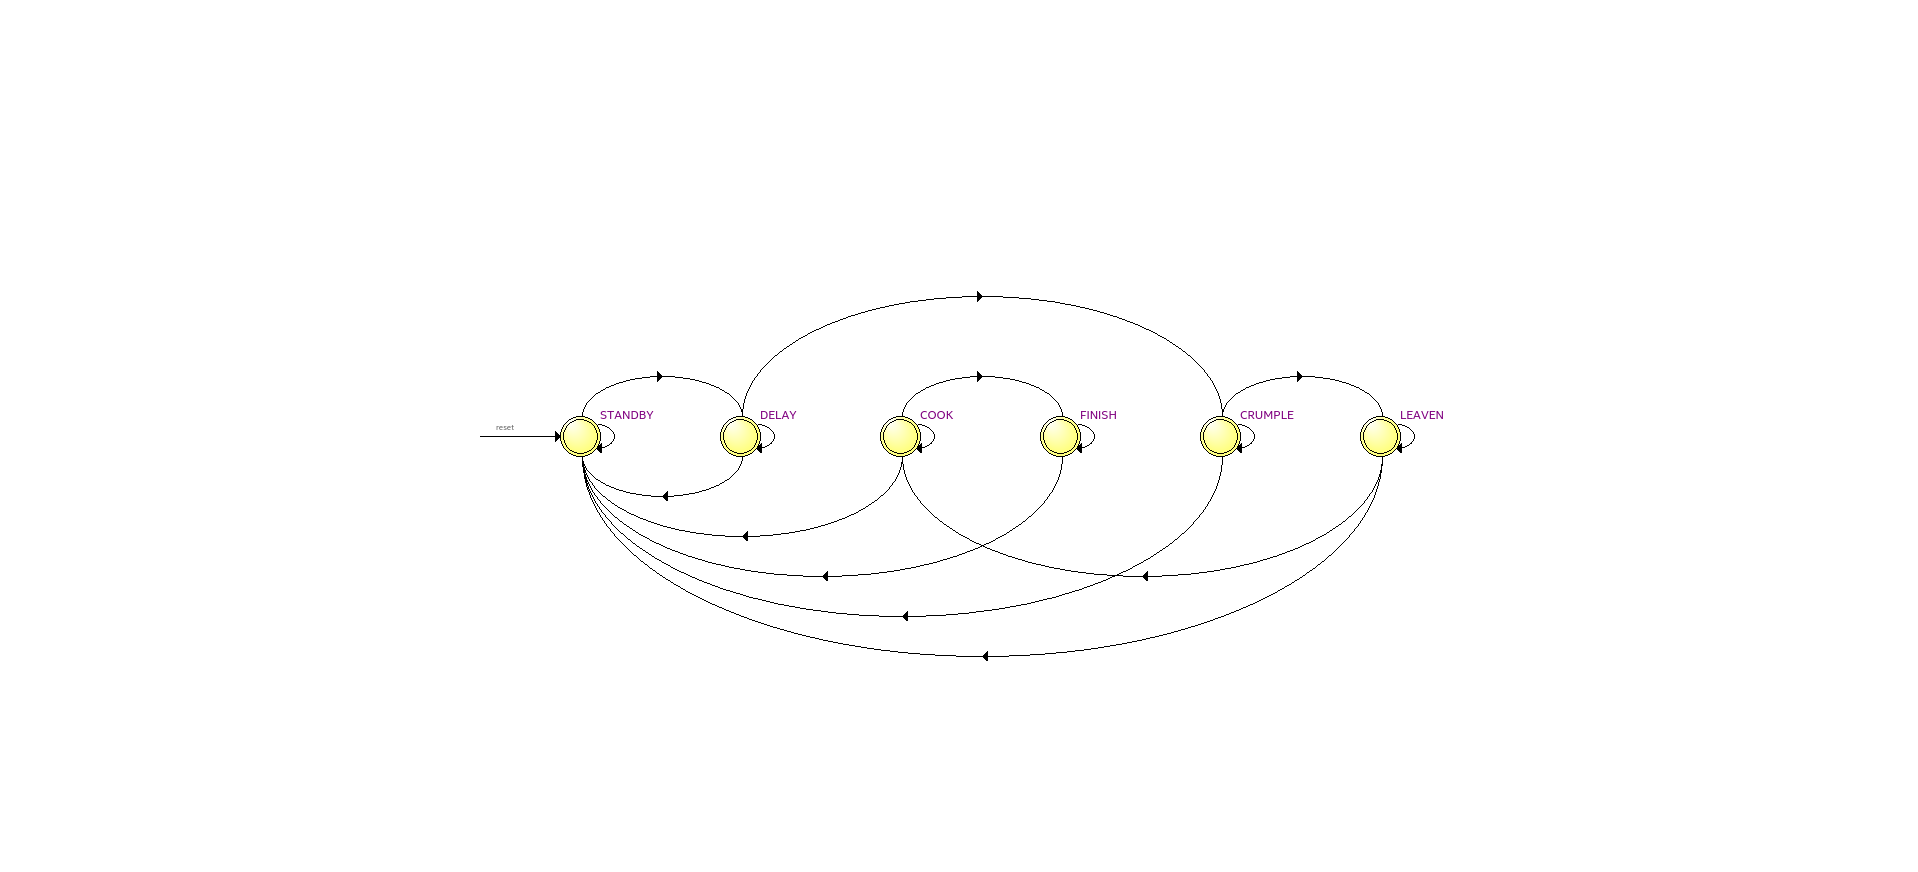
\includegraphics[scale=0.4]{FSM}
        \caption{Máquina de estados presente no projeto}
        \label{fig:fsm}
    \end{figure}

    \begin{itemize}
        \label{finite-states}
        \item \textbf{STANDBY} - Este estado é o estado inicial da máquina. \ Por defeito, permite selecionar o programa que o utilizador pretende, adicionar tempo extra de cozedura ou adicionar tempo de espera total da máquina. \ Este estado será ativado quando o utilizador clica no botão de reset ou o pão a ser processado acaba o seu tempo de cozedura;
        \item \textbf{DELAY} - Após iniciar a máquina, ela transita para este estado, mesmo que nenhum tempo extra tenha sido introduzido a máquina irá fazer a verificação e avançara para o estado seguinte.\ A verificação é feita iniciando o temporizador com o tempo total das 3 etapas para fabricar o pão, acrescentado com o tempo extra pre definido que pode ser zero.\ A saída do temporizador é lida pela máquina e é feita a verfificação para proceder para o estado seguinte;
        \item \textbf{CRUMPLE} - Terminando o tempo de espera, o seu programa dará início.\ Chegando a este estado, a máquina acenderá os \textit{leds}: LEDG0, LEDG1, LEDG2 e LEDR0 para mostrar as 3 etapas e que a máquina está ligada respetivamente.\ Assim que o tempo desta etapa termina avançara de estado.
        \item \textbf{LEAVEN} - Sendo a  segunda etapa para a fabricação do pão e desliga um \textit{LED} verde para mostrar que terminou uma etapa.\ Tal como o estado anterior, a máquina espera pelo temporizador para poder transitar para o estado seguinte.
        \item \textbf{COOK} - Etapa final onde realiza o mesmo que o anterior desligando um outro \textit{LED} verde e aguarda para avançar de estado.
        \item \textbf{FINISH} - Fim do programa, é desligado o \textit{LED} verde restante e aguarda 2 segundos para apagar o \textit{LED} vermelho regressando ao estado STANDBY para aceitar um novo pedido.
    \end{itemize}

     Destaca-se também o botão de \textit{start/stop}, que permite interromper o programa e resumir a qualquer momento e o \textit{reset} força a máquina a voltar ao início.

    % Manual do Utilizador
    \newpage
    \section{Manual do Utilizador}\label{sec:manualUtilizador}
        Nesta secção será apresentado um manual de utilizador para o funcionamento da máquina de pão.

    \begin{multicols}{2}
        \begin{figure}[H]
            \centering
            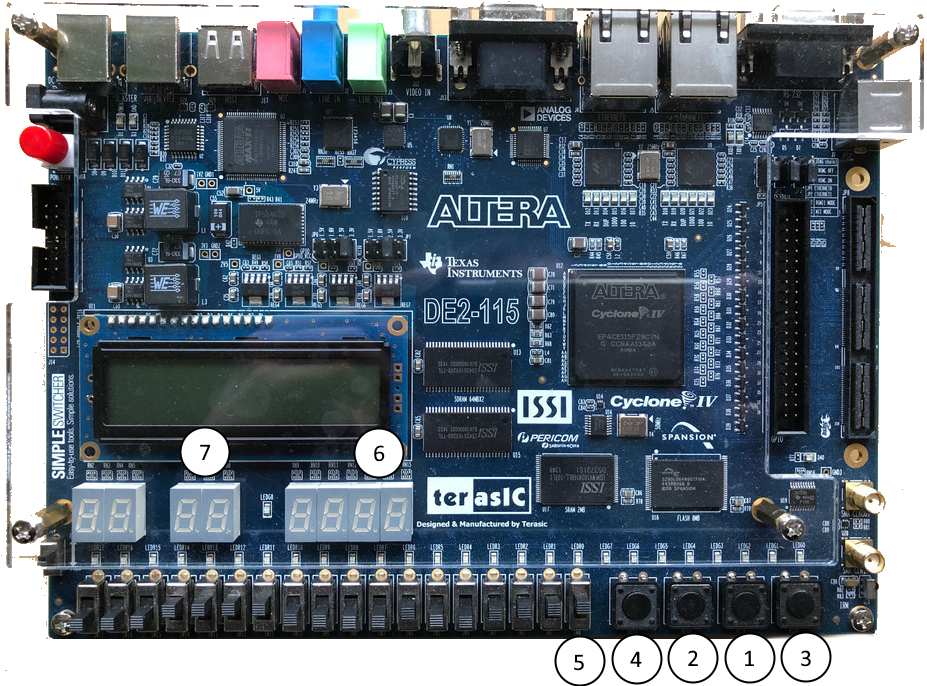
\includegraphics[scale=0.3]{FPGA}
            \caption{Imagem representativa da placa Terasic Altera DE2-115}
            \label{fig:fpga}
        \end{figure}

        \section*{LEGENDA:}
        \begin{enumerate}
            \item \textbf{KEY1} - Função \textit{start/stop} da máquina;
            \item \textbf{KEY2} - Botão \textit{reset} da máquina;
            \item \textbf{KEY0} - Botão para adicionar tempo extra de cozedura;
            \item \textbf{KEY3} - Botão para adicionar tempo de espera ao tempo total da máquina;
            \item \textbf{SW0} - Botão de seleção do programa (rústico ou normal);
            \item \textbf{HEX0/HEX1} - \textit{Displays} de 7 segmentos para mostrar o tempo total da máquina;
            \item \textbf{HEX4} - \textit{Display} de 7 segmentos  com o propósito de mostrar o tempo extra de cozedura;
        \end{enumerate}
    \end{multicols}

    % Conclusion
    \section{Conclusão}\label{sec:conclusao}
        Com este projeto foi possível aprofundar os conhecimentos adquiridos nas aulas teóricas e práticas da unidade curricular de \acs{lsd}. \ Com o projeto que foi atribuído aos autores, foi possível desenvolver vários componentes necessários para o projeto na linguagem \acs{vhdl}, como um contador decrescente, um temporizador, um \textit{button toggler}, entre outros. \\
        Utilizando os componentes desenvolvidos, foi possível desenvolver uma máquina de estados finitos que comanda o funcionamento de uma máquina de pão. \\
        \par Os autores também consideram que o projeto foi concluído com sucesso, tendo sido alcançado todos os objetivos propostos no guião com eficácia.

    \subsection{Autoavaliação}\label{subsec:autoavaliacao}
        A autoavaliação dos autores deste projeto é a seguinte:
        \begin{itemize}
            \item \authorjp - 50\%
            \item \authorrg - 50\%
        \end{itemize}



    % Acronyms
    \newpage
    \section*{Acrónimos}
    \begin{acronym}
        \acro{vhdl}[VHDL]{Very High-Speed Integrated Circuit Hardware Description Language}
        \acro{lsd}[LSD]{Laboratório de Sistemas Digitais}
    \end{acronym}

    \begin{flushright}
        \today
    \end{flushright}
\end{document}